Die Probanden haben den UEQ bzgl. der Authentisierung einmal für das traditionelle 
TOTP-Verfahren und einmal für Blue TOTP ausgefüllt. Es sollte nur die Authentisierung 
mit dem jeweiligen Verfahren beurteilt werden, also auch die Handhabung der TOTP-App. 
Das Design von Website bei der Anmeldung sollte kein Bestandteil der Beurteilung sein.
\\\\
In Abb. \ref{fig: studie ergebnisse auth ueq bt trad single} sind die Mittelwerte jedes Gegensatzpaares dargestellt.
\begin{figure}
    \centering
    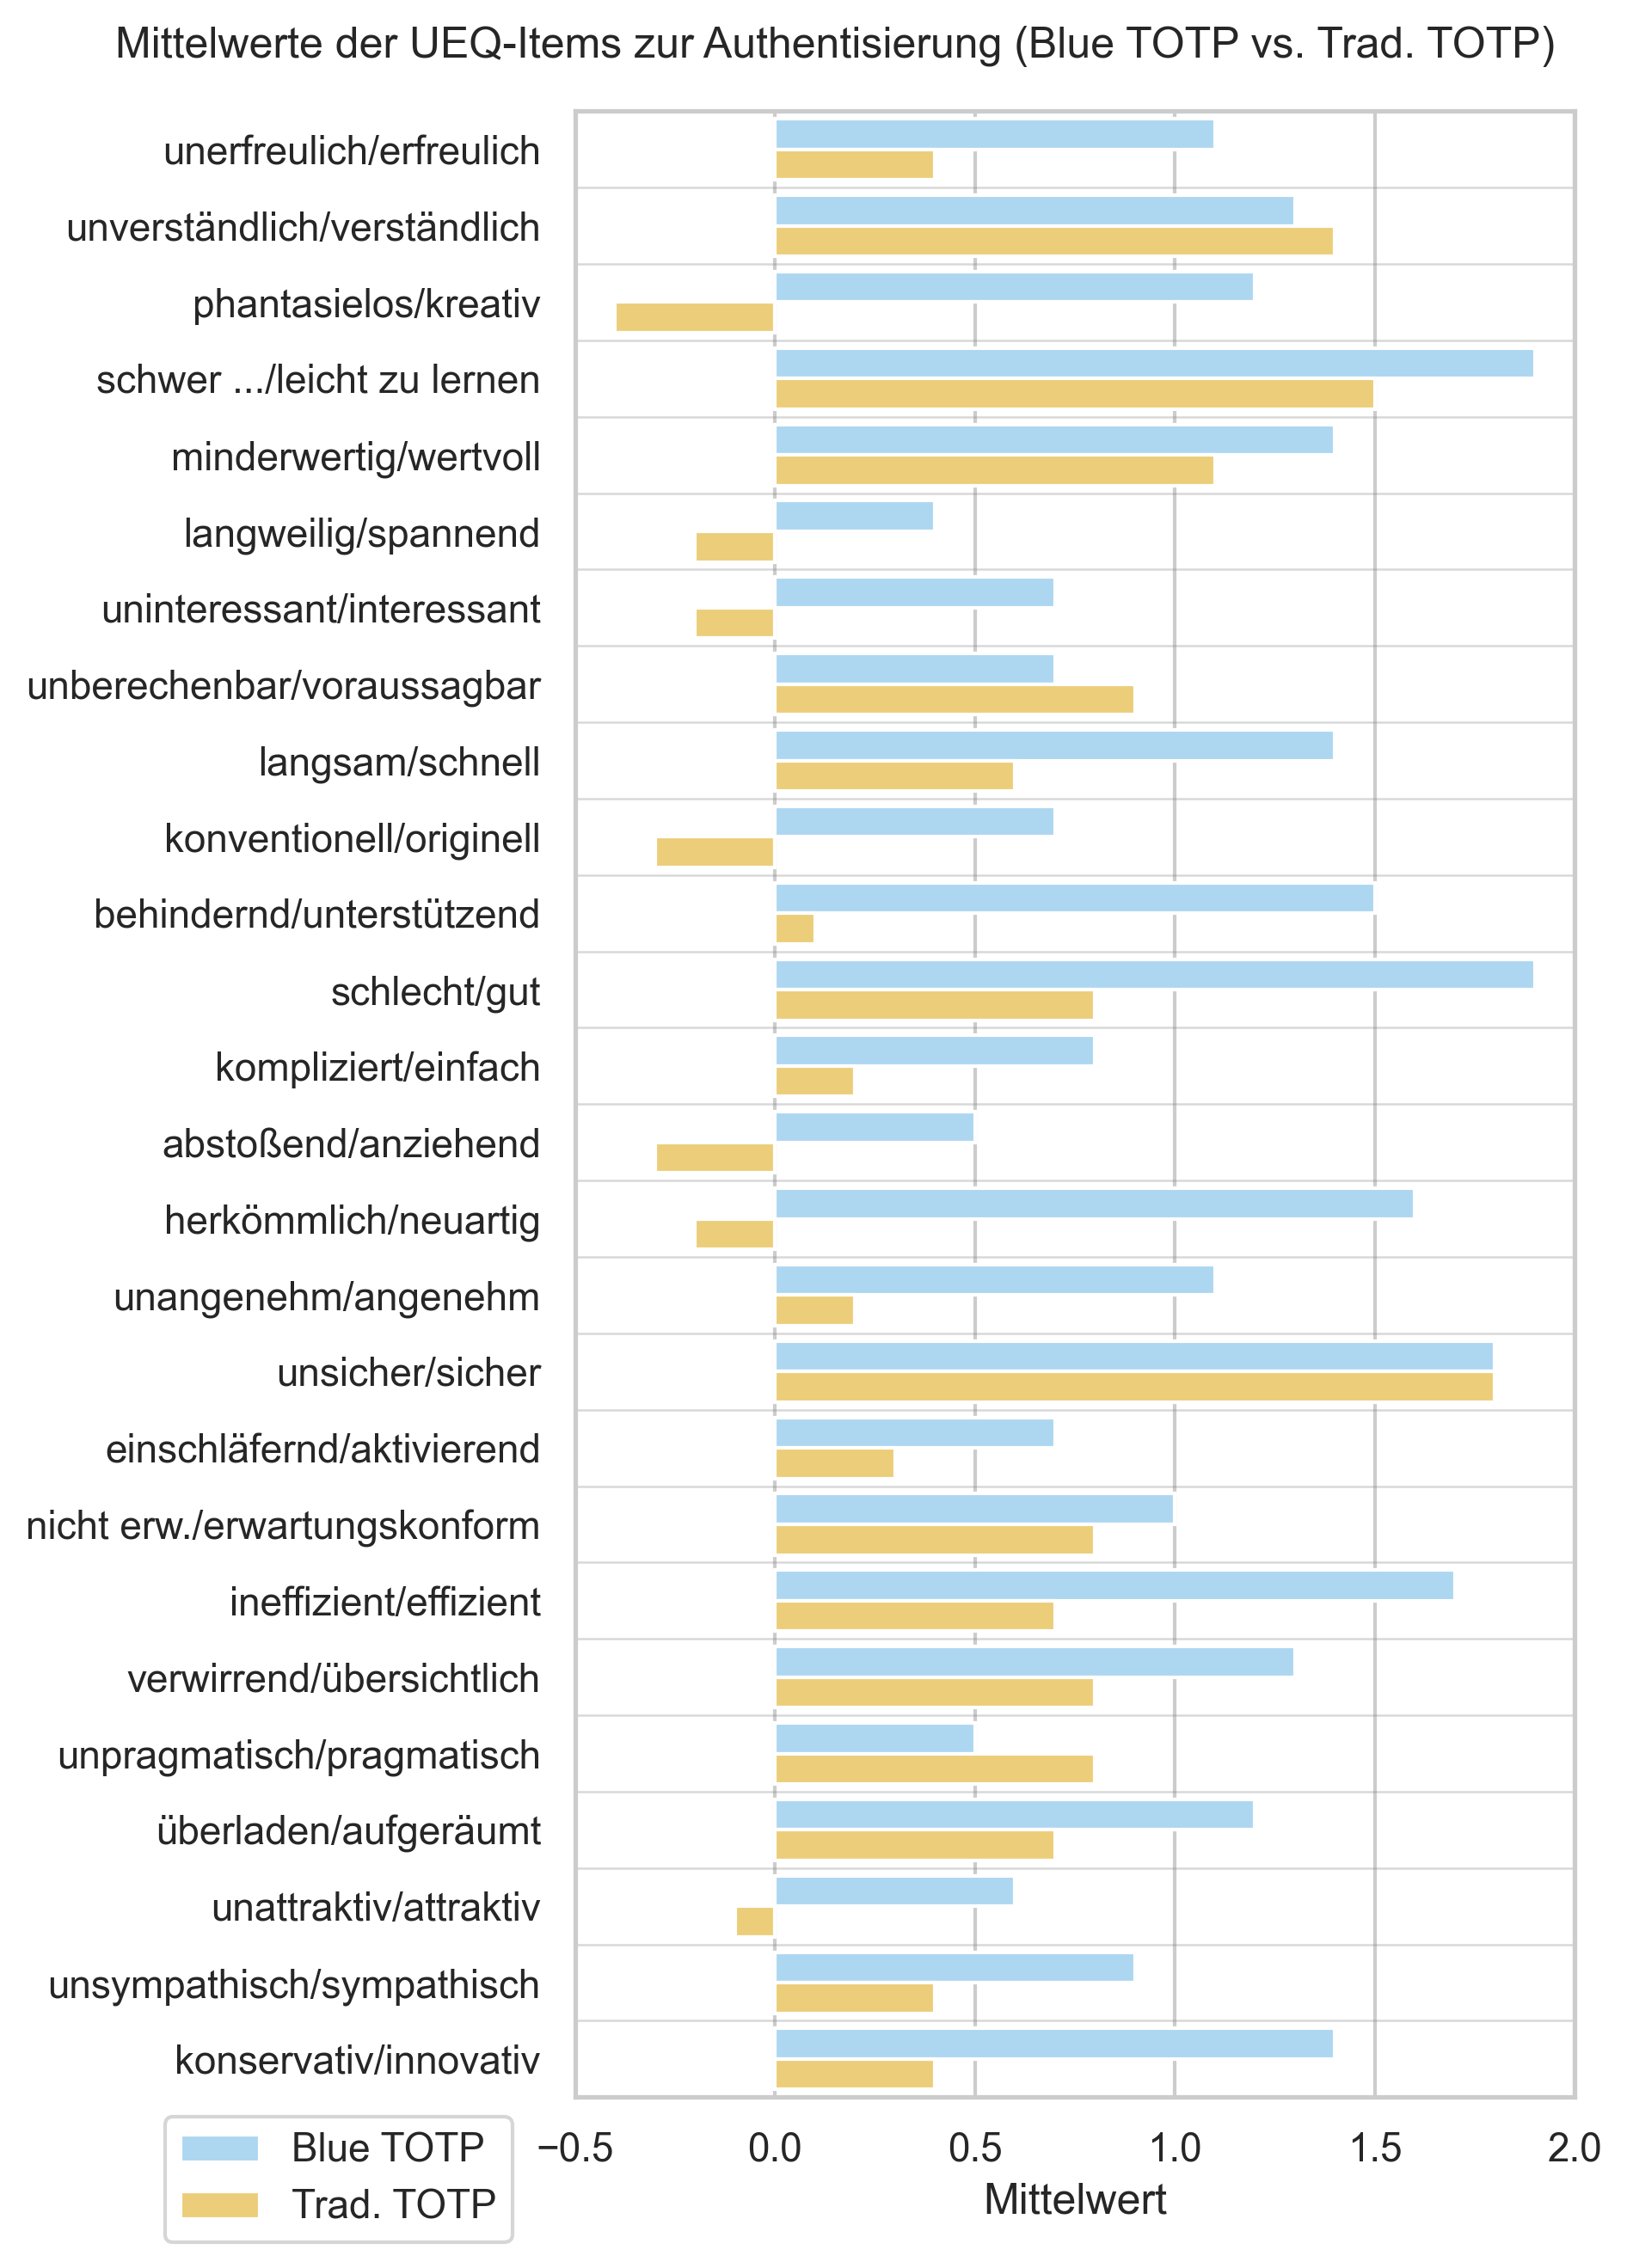
\includegraphics[width=0.65\linewidth]{data_processing/questionaires/results/from_ueq_excel/ueq_single_means_bt_trad.png}
    \caption[Mittelwert pro Gegensatzpaar des UEQ (Blue TOTP vs. trad. TOTP)]{Mittelwert pro Gegensatzpaar des UEQ (Blue TOTP vs. trad. TOTP)}
    \label{fig: studie ergebnisse auth ueq bt trad single}
\end{figure}
Es ist auffällig, dass viele Mittelwerte der hedonischen Gegensatzpaare (zugehörig zu 
Stimulation und Originalität) gegensätzlich sind.
Beispiele sind \glqq phantasielos/kreativ\grqq{}, \glqq langweilig/spannend\grqq{} 
und \glqq herkömmlich/neuartig\grqq{}. 
Bei diesen hedonischen Paaren liegt der Mittelwert für das traditionelle 
TOTP-Verfahren überwiegend im negativen Bereich zwischen $0$ und $-0{,}5$. Generell 
erkennt man, dass Blue TOTP überwiegend einen höheren Mittelwert erreicht als das 
traditionelle Verfahren. Einige dieser Gegensatzpaare sind \glqq unerfreulich/
erfreulich\grqq{} mit $\bar{x}_{Blue} = 1{,}1$ zu $\bar{x}_{Trad} = 0{,}4$ oder \glqq 
langsame/schnell\grqq{} mit $\bar{x}_{Blue} = 1{,}4$ zu $\bar{x}_{Trad} = 0{,}6$. 
Auch die für Blue TOTP positive Differenz bei \glqq behindernd/unterstützend\grqq{} 
($1{,}4$) sowie \glqq unangenehmen/angenehm\grqq{} ($0{,}9$) ist bemerkenswert. 
Nicht sonderlich unerwartet ist der Gleichstand bei \glqq unsicher/sicher\grqq{}. Nur 
bei den Kriterien, wie pragmatisch und verständlich es ist, steht Blue TOTP dem 
traditionellen Verfahren nach mit einer geringen Differenzen von $\le 0{,}3$.
\\\\
Der Vergleich beider Systeme bzgl. der UEQ-Skalen ist in Abb. \ref{fig: studie 
ergebnisse auth ueq overview} dargestellt.
\begin{figure}
    \centering
    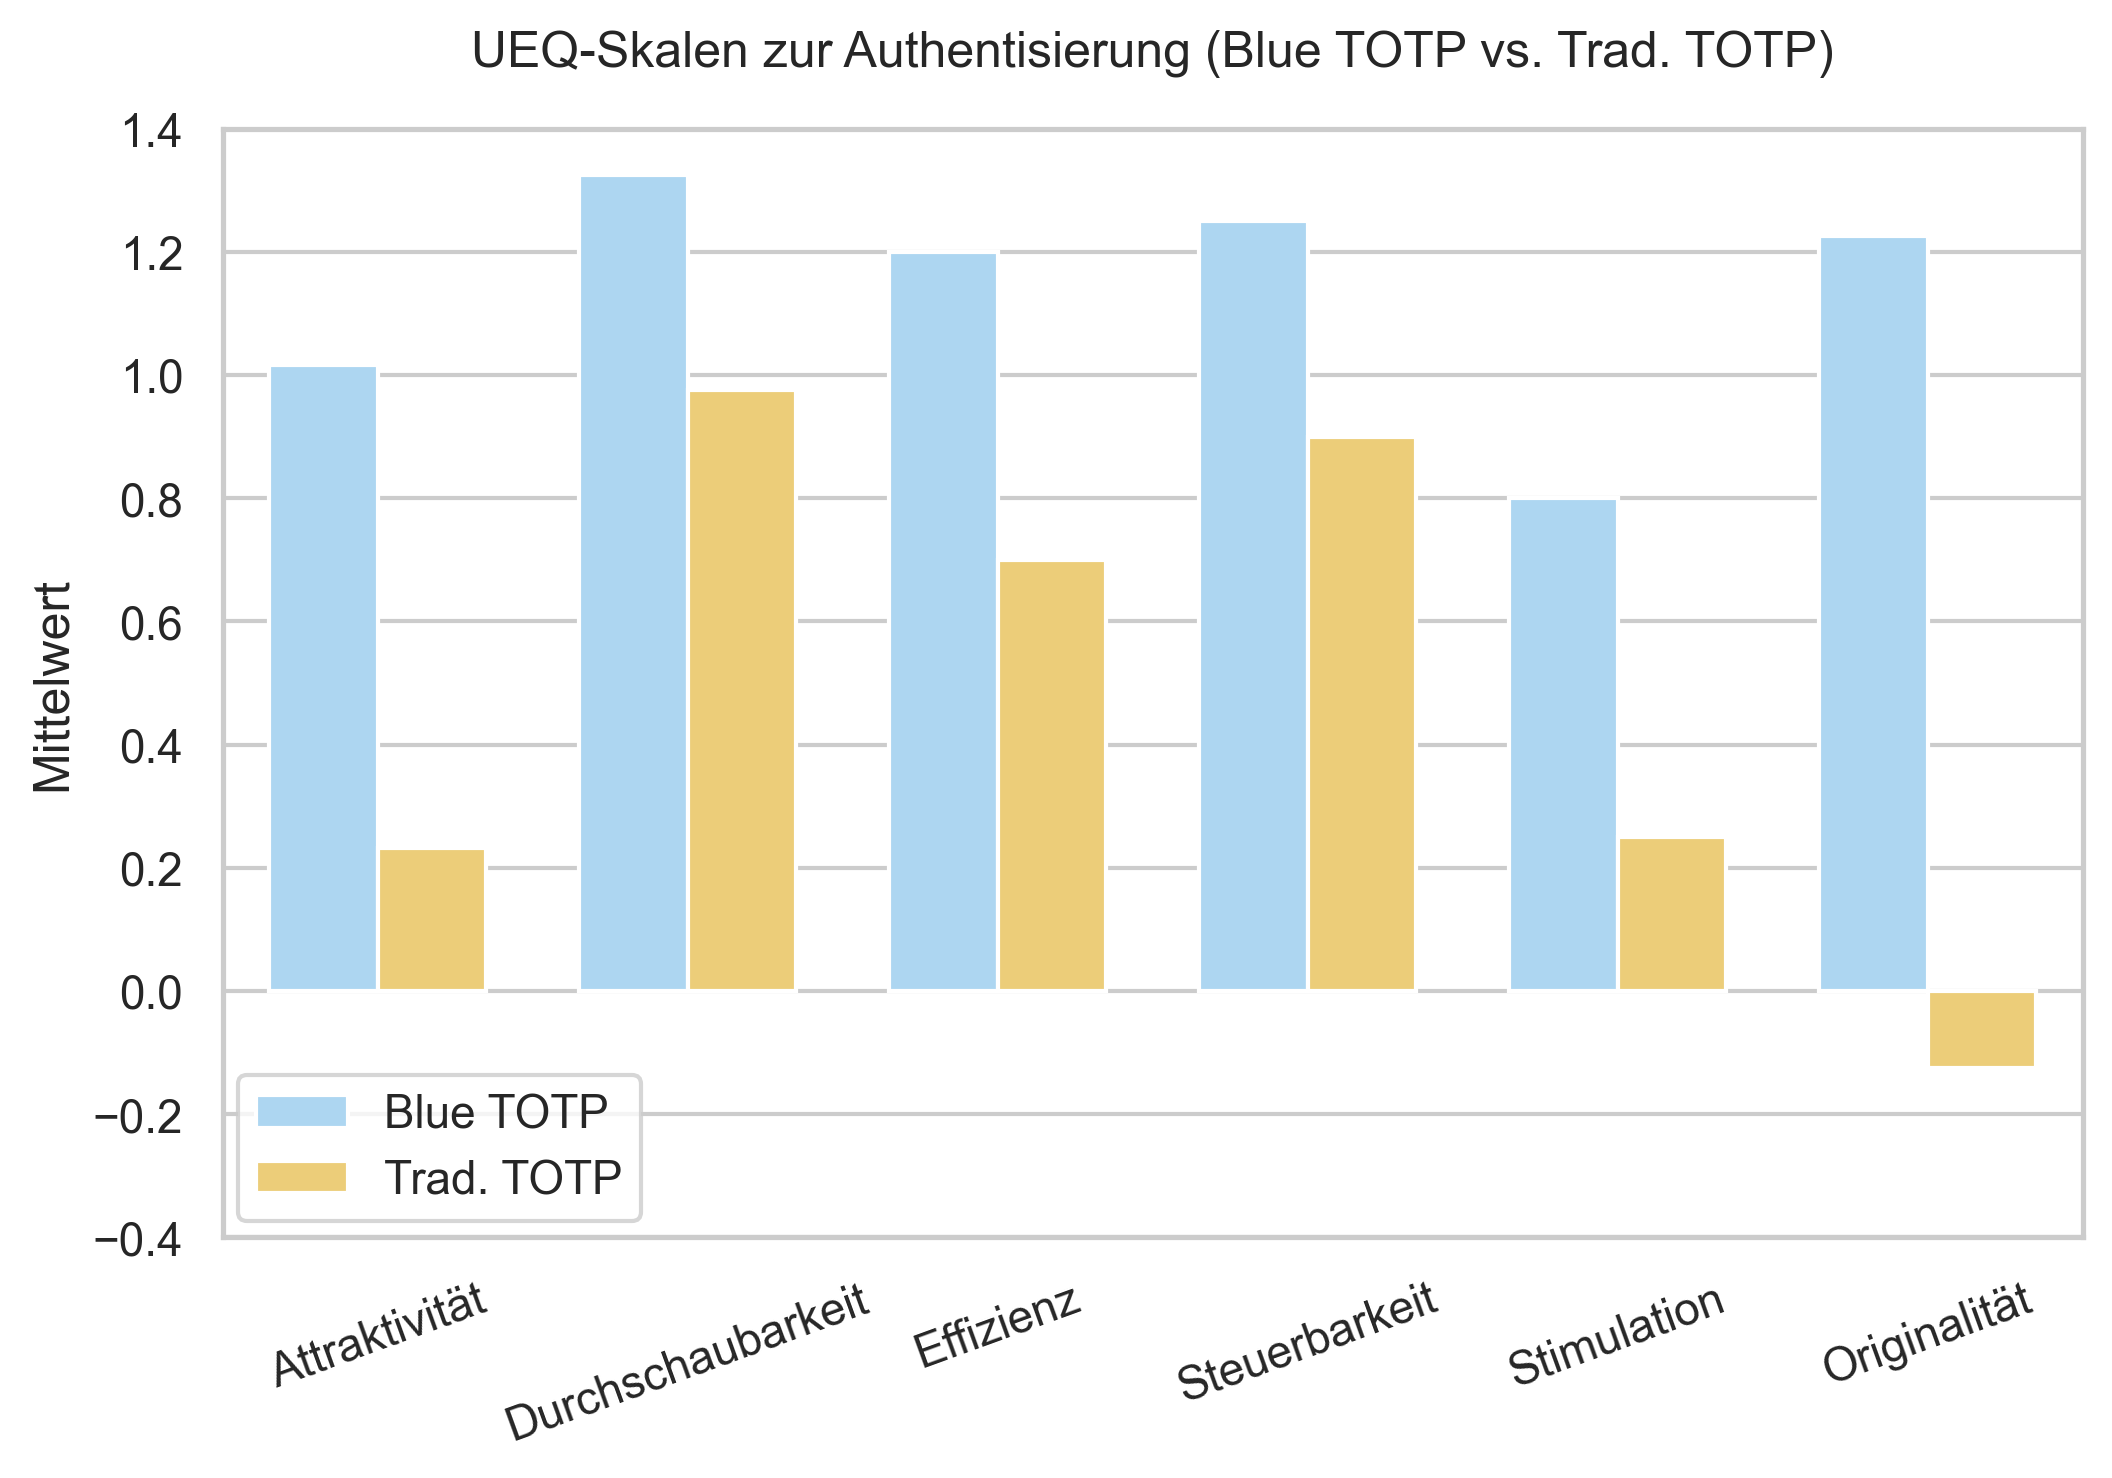
\includegraphics[width=0.75\linewidth]{data_processing/questionaires/results/from_ueq_excel/ueq_overview_bt_trad.png}
    \caption[Vergleich der UEQ-Skalen zur Authentisierung (Blue TOTP vs. trad. TOTP)]{Vergleich der UEQ-Skalen zur Authentisierung (Blue TOTP vs. trad. TOTP)}
    \label{fig: studie ergebnisse auth ueq overview}
\end{figure}
Statistische Signifikanz für $\alpha = 0{,}05$ zwischen Blue TOTP und dem trad. TOTP wurde bei den Skalen Attraktivität ($p = 0{,}0183$) und Originalität ($p = 0{,}004$) erreicht (t-Test). Dazu wurde ein Zweistichproben-t-Test verwendet. Wie bereits bei den einzelnen Gegensatzpaaren beobachtet, übertrifft Blue TOTP das 
traditionelle Verfahren im Mittelwert jeder Skala. Die höchste Differenz bildet sich 
in der Originalität mit $1{,}1$. Auch die Stimulation ist um einen Wert von fast $0{,}
6$ höher. Allerdings sollte man beachten, dass laut \textcite{Schrepp} der positive 
Bewertungsbereich erst bei $0{,}8$ (aufsteigend) beginnt. Demnach ist Stimulation bei 
Blue TOTP nichts außergewöhnliches. Auch sollte man sich des potentiellen Minimums 
von $-3$ bzw. des Maximums von $3$ bewusst sein. Die anderen Skalen hinsichtlich der 
Forschungsfragen sind von mehr Bedeutung. Damit ist vor allem die 
Attraktivität und die Effizienz gemeint. Bei der Attraktivität ist zu Gunsten von 
Blue TOTP eine Verfünffachung von ca. $0{,}2$ auf $1{,}0$ zu verzeichnen. Auch bei 
der Effizienz ist ein positiver Effekt zu verzeichnen. Im Vergleich zum 
traditionellen Verfahren erstreckt sich jede Skala von Blue TOTP (mit Ausnahme der 
Stimulation) bis deutlich über die Grenze zwischen dem neutralen und positiven 
Bewertungsbereich.